\subsection*{Problema 04}

\textbf{Enunciado:} Calcular la integral:\\
$\int \dfrac{2x+2}{x^2 - 4x + 9} \, dx$

\textbf{Solución:} \
Siguiendo las indicaciones, buscamos que el numerador contenga la derivada del denominador, la cual es $D_x(x^2 - 4x + 9) = 2x - 4$. 

Manipulamos algebraicamente el numerador sumando y restando $4$:
\begin{align*}
2x + 2 &= 2x - 4 + 4 + 2 \\
&= (2x - 4) + 6
\end{align*}

Sustituimos esta expresión en la integral original y la separamos en dos partes:
\begin{align*}
I &= \int \dfrac{(2x - 4) + 6}{x^2 - 4x + 9} \, dx \\
&= \int \dfrac{2x - 4}{x^2 - 4x + 9} \, dx \\
&\quad + \int \dfrac{6}{x^2 - 4x + 9} \, dx
\end{align*}

Para la primera integral ($I_1$), aplicamos el método de sustitución haciendo $u = x^2 - 4x + 9$, de donde $du = (2x - 4) \, dx$:
\begin{align*}
I_1 &= \int \dfrac{du}{u} = \ln|u| \\
&= \ln|x^2 - 4x + 9|
\end{align*}

Para la segunda integral ($I_2$), completamos el trinomio cuadrado en el denominador:
\begin{align*}
x^2 - 4x + 9 &= (x^2 - 4x + 4) - 4 + 9 \\
&= (x - 2)^2 + 5
\end{align*}

Sustituimos $I_2$ utilizando la fórmula de integración $\int \dfrac{1}{u^2 + a^2} \, du = \dfrac{1}{a}\arctan\left(\dfrac{u}{a}\right)$:
\begin{align*}
I_2 &= \int \dfrac{6}{(x-2)^2 + 5} \, dx \\
&= \dfrac{6}{\sqrt{5}} \arctan\left(\dfrac{x - 2}{\sqrt{5}}\right)
\end{align*}

Finalmente, unimos ambas soluciones y añadimos la constante de integración $C$:
\begin{align*}
I &= \ln(x^2 - 4x + 9) \\
&\quad + \dfrac{6}{\sqrt{5}} \arctan\left(\dfrac{x - 2}{\sqrt{5}}\right) + C
\end{align*}

\begin{figure}[H]
	\centering
	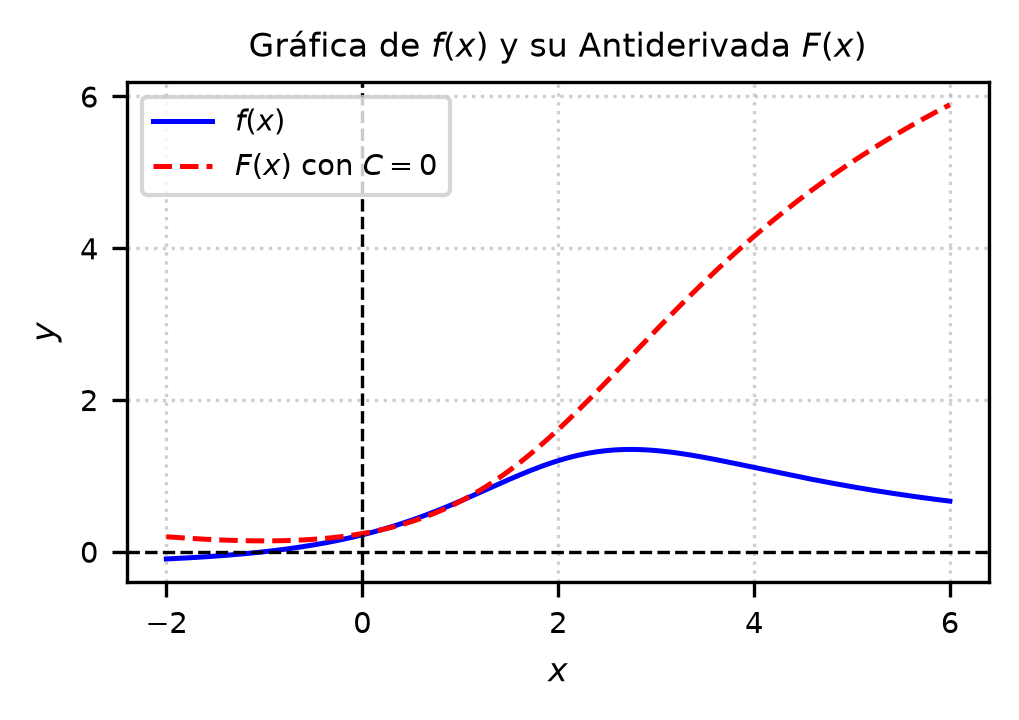
\includegraphics[width=\columnwidth]{semana_03/graficas/SEM03_P04_grafica.png}
	\caption{Representación gráfica de $f(x)$ y su antiderivada $F(x)$ evaluada para la constante de integración $C = 0$ (Problema 04).}
	\label{fig:problema04}
\end{figure}
